
%(BEGIN_QUESTION)
% Copyright 2012, Tony R. Kuphaldt, released under the Creative Commons Attribution License (v 1.0)
% This means you may do almost anything with this work of mine, so long as you give me proper credit

A newly-installed pH measurement system does not seem to be measuring the pH of the process liquid accurately.  The indicating controller's display does not match the display of the hand-held pH meter used by an operator:

$$\includegraphics[width=15.5cm]{i00976x01.eps}$$

The calibrated range of the 4-wire pH transmitter is supposed to be 2 to 12 pH, with a 4 to 20 mA signal output range.  An instrument technician begins to diagnose the problem by taking a loop calibrator and measuring the current signal being sent to the indicating controller.  The loop calibrator registers 15.43 milliamps.

\vskip 10pt

Based on this information, determine where the problem is in this system.  Also, show how the loop calibrator could be connected to the wiring to measure the loop current (specifying the proper calibrator mode as well).

\vskip 20pt \vbox{\hrule \hbox{\strut \vrule{} {\bf Suggestions for Socratic discussion} \vrule} \hrule}

\begin{itemize}
\item{} Review the problem-solving tips listed in Question 0 and apply them to this problem.
\item{} A problem-solving technique useful for making proper connections in pictorial circuit diagrams is to first identify the directions of all DC currents entering and exiting component terminals, as well as the respective voltage polarity marks (+,$-$) for those terminals, based on your knowledge of each component acting either as an electrical {\it source} or an electrical {\it load}.  Discuss and compare how these arrows and polarity marks simplify the task of properly connecting wires between components. 
\item{} If the technician had no test equipment except for a voltmeter, could a good diagnostic test still be made in this system?
\item{} Identify where you could install a rectifying diode in this circuit to allow convenient measurement of loop current.
\end{itemize}

\underbar{file i00976}
%(END_QUESTION)





%(BEGIN_ANSWER)

15.43 milliamps of current equates to a percentage value of 71.44\%:

$${15.43 - 4 \over 16} \times 100\% = 71.44\%$$

This, in turn, represents a pH value of:

$$0.7144 \times (12 - 2) + 2 = 9.144 \hbox{ pH}$$

\vskip 10pt

This largely agrees with the controller's display, which tells us there is a {\it slight} calibration error on either the part of the controller or the resistor.  The huge discrepancy between this calculated pH value and what the hand-held pH meter registers, however, tells us there is either a problem with the pH transmitter, the pH probe, or the hand-held meter.  We may further conclude there is no problem with the 250 $\Omega$ resistor or the indicating controller.
 
\vskip 10pt

The proper setup of the loop calibrator is to place it into the ``READ'' (measure) mode so that it functions as a simple ammeter, then connect it in series with the output of the 4-wire transmitter.  This may be done either with the indicating controller still in the circuit, or removed from the circuit.

%(END_ANSWER)





%(BEGIN_NOTES)

\filbreak \vskip 20pt \vbox{\hrule \hbox{\strut \vrule{} {\bf Virtual Troubleshooting} \vrule} \hrule}

$$\includegraphics[width=15.5cm]{i00976x02.eps}$$

\noindent
{\bf Predicting the effect of a given fault:} present each of the following faults to the students, one at a time, having them comment on all the effects each fault would produce.

\begin{itemize}
\item{} Wire E-A failing open
\item{} Wire F-B failing open
\item{} Wire G-C failing open
\item{} Wire H-D failing open
\item{} Resistor failing open
\item{} 28 VDC power supply dying
\end{itemize}


\vskip 10pt


\noindent
{\bf Determining the utility of given diagnostic tests:} imagine the resistor fails open in this circuit (but don't tell this to students!).  Present the operator's observation(s) to the students, have them consider possible faults and diagnostic strategies, and then propose the following diagnostic tests one by one.  Have students rate the value of each test, determining whether or not each test would give us useful information (i.e. tell us something we don't already know).  Also have students describe what result in particular might be the most informative for any of these tests, because the same test might yield conclusive or inconclusive results depending on the fault:

\begin{itemize}
\item{} Operator sees the controller PV display registering 105\% (12.5 pH)
\item{} Measure $V_{AD}$
\item{} Measure $V_{EH}$
\item{} Measure current at terminal B
\item{} Measure voltage at input terminals of controller
\item{} Measure solution pH with a hand-held meter
\item{} Place controller in manual mode and change the output value
\end{itemize}


\vskip 10pt


\noindent
{\bf Diagnosing a fault based on given symptoms:} imagine the wire connecting terminals F and B breaks open in this circuit (but don't tell this to students!).  Present the operator's observation(s) to the students, have them consider possible faults and diagnostic strategies, and then tell them the results of tests they propose based on the following symptoms, until they have properly identified the nature and location of the fault:

\begin{itemize}
\item{} Operator sees the controller PV display registering -25\% (-0.5 pH)
\item{} $V_{AD}$ = 28 VDC
\item{} $V_{EH}$ = 28 VDC
\item{} $V_{FG}$ = 28 VDC
\item{} $V_{BC}$ = 0 VDC
\end{itemize}

%INDEX% Calibration errors, identifying
%INDEX% Electronics review: 4-20 mA loop calibrator (test equipment)
%INDEX% Pictorial circuit review (4-20 mA loop)

%(END_NOTES)


